%\documentclass[leqno,12pt]{amsart}
\documentclass[11pt]{article}
\oddsidemargin=0in \evensidemargin=0in
\textwidth=6.5in \textheight=8.5in

%\usepackage{hyperref}

\usepackage[dvips]{pict2e}
\usepackage{amssymb,enumerate, latexsym, mathrsfs, mdwlist}
\usepackage{amsmath,amsthm}
\usepackage[all,cmtip]{xy}
\usepackage{amsfonts, fullpage, fancyhdr, qtree, amsmath, tipa, amssymb, url, subfigure, enumitem, setspace, mathrsfs, verbatim}
%\usepackage{amsfonts, fancyhdr, qtree, amsmath, tipa, amssymb, url, subfigure, enumitem, setspace, mathrsfs, verbatim, color}
\usepackage{stmaryrd}
\usepackage{appendix}
%\usepackage{xypic}
%\usepackage[pdftex]{graphicx}
\usepackage{leftidx}

%----------------------------------------------------------------------%

%\renewcommand{\appendixname}{Example}

%\swapnumbers
\theoremstyle{definition}
\newtheorem{nul}{}[section]
\newtheorem{dfn}[nul]{Definition}
\newtheorem{axm}[nul]{Axiom}
\newtheorem{rmk}[nul]{Remark}
\newtheorem{cnstr}[nul]{Construction}
\newtheorem{ntn}[nul]{Notation}
\newtheorem{exm}[nul]{Example}
\newtheorem{ctrexm}[nul]{Counterexample}
\newtheorem{rec}[nul]{Recollection}
\newtheorem{exr}[nul]{Exercise}
\newtheorem{wrn}[nul]{Warning}
\newtheorem*{dfn*}{Definition}
\newtheorem*{axm*}{Axiom}
\newtheorem*{ntn*}{Notation}
\newtheorem*{exm*}{Example}
\newtheorem*{exr*}{Exercise}
\newtheorem*{int*}{Intuition}
\newtheorem*{qst*}{Question}

\theoremstyle{plain}




\newtheorem{sch}[nul]{Scholium}
\newtheorem{thm}[nul]{Theorem}
\newtheorem{prop}[nul]{Proposition}
\newtheorem{lem}[nul]{Lemma}
\newtheorem{sublem}{Lemma}[nul]
\newtheorem{por}[nul]{Porism}
\newtheorem{cnj}[nul]{Conjecture}
\newtheorem{cor}{Corollary}[nul]
\newtheorem*{thm*}{Theorem}
\newtheorem*{mainthm*}{Universal Additivity Theorem}
\newtheorem*{structurethm*}{Structure Theorem}
\newtheorem*{prop*}{Proposition}
\newtheorem*{cor*}{Corollary}
\newtheorem*{lem*}{Lemma}
\newtheorem*{cnj*}{Conjecture}

\numberwithin{equation}{nul}

    \newtheoremstyle{TheoremNum}
      %  {\topsep}{\topsep}              %%% space between body and thm
			  {2mm}{2mm}              %%% space between body and thm
        {\itshape}                      %%% Thm body font
        {}                              %%% Indent amount (empty = no indent)
        {\bfseries}                     %%% Thm head font
        {.}                             %%% Punctuation after thm head
        { }                             %%% Space after thm head
        {\thmname{#1}\thmnote{ \bfseries #3}}%%% Thm head spec
    \theoremstyle{TheoremNum}
    \newtheorem{thmn}{Theorem}

%----------------------------------------------------------------------%

%\frenchspacing

%----------------------------------------------------------------------%

\DeclareMathOperator{\Aut}{\text{Aut}}
\DeclareMathOperator{\Tr}{\text{Tr}}
\DeclareMathOperator{\Res}{\text{Res}}
\DeclareMathOperator{\im}{\text{im}}
\DeclareMathOperator*{\colim}{\text{colim}}
\DeclareMathOperator{\Map}{\text{Map}}
\DeclareMathOperator{\cofiber}{\text{cofiber}}
\DeclareMathOperator{\fiber}{\text{fiber}}
\DeclareMathOperator{\Hom}{\text{Hom}}
\DeclareMathOperator{\Skel}{\text{Skel}}
\DeclareMathOperator*{\hocolim}{\text{hocolim}}
\DeclareMathOperator*{\holim}{\text{holim}}

\DeclareMathOperator{\C}{\mathcal{C}}
\DeclareMathOperator{\CP}{\mathbb{CP}}
\DeclareMathOperator{\Z}{\mathbb{Z}}
\DeclareMathOperator{\E}{\mathbb{E}}
\DeclareMathOperator{\Q}{\mathbb{Q}}
\DeclareMathOperator{\m}{\mathfrak{m}}
\DeclareMathOperator{\G}{\mathbb{G}}
\DeclareMathOperator{\F}{\mathbb{F}}
\DeclareMathOperator{\J}{\mathcal{J}}
\DeclareMathOperator{\cG}{\mathcal{G}}
\DeclareMathOperator{\cF}{\mathcal{F}}
\DeclareMathOperator{\cS}{\mathcal{S}}
\DeclareMathOperator{\Ring}{\textbf{Ring}}
\DeclareMathOperator{\Aff}{\textbf{Aff}}
\DeclareMathOperator{\Spec}{\text{Spec}}
\DeclareMathOperator{\Ext}{\text{Ext}}
\DeclareMathOperator{\nil}{\text{nil}}
\DeclareMathOperator{\Gr}{\textbf{Gr}}
\DeclareMathOperator{\Fil}{\textbf{Fil}}
\DeclareMathOperator{\Cofil}{\textbf{Cofil}}
\DeclareMathOperator{\Fun}{\text{Fun}}
\DeclareMathOperator{\Alg}{\text{Alg}}
\DeclareMathOperator{\Sp}{\text{Sp}}
\DeclareMathOperator{\Spaces}{\mathcal{S}}
\DeclareMathOperator{\S0}{\mathbb{S}}



\DeclareMathOperator{\smsh}{\wedge}
\DeclareMathOperator{\uBPn}{\underline{BP\langle n \rangle}}
\DeclareMathOperator{\uE}{\underline{E}}
\DeclareMathOperator{\uHom}{\underline{\Hom}}
\DeclareMathOperator{\uMU}{\underline{MU}}

\newcommand\myatop[2]{\genfrac{}{}{0pt}{}{#1}{#2}}
\newcommand\BPn{BP\langle n \rangle}
\newcommand\HFp{\text{H}\mathbb{F}_p}
\newcommand\HZp{\text{H}\mathbb{Z}_{(p)}}
\newcommand\HFtwo{\text{H}\mathbb{F}_2}
\newcommand\HZtwo{\text{H}\mathbb{Z}_{(2)}}

%----------------------------------------------------------------------%

\usepackage{tikz}
\usetikzlibrary{matrix,arrows,decorations}
\usepackage{tikz-cd}

%\pgfdeclaredecoration{single line}{initial}{\state{initial}[width=\pgfdecoratedpathlength-1sp]{\pgfpathmoveto{\pgfpointorigin}}\state{final}{\pgfpathlineto{\pgfpointorigin}}} 

\newcommand{\fromto}[2]{{#1}\ \tikz[baseline]\draw[>=stealth,->](0,0.5ex)--(0.5,0.5ex);\ {#2}}
\newcommand{\into}[2]{{#1}\ \tikz[baseline]\draw[>=stealth,right hook->](0,0.5ex)--(0.5,0.5ex);\ {#2}}
\newcommand{\onto}[2]{{#1}\ \tikz[baseline]\draw[>=stealth,->>](0,0.5ex)--(0.5,0.5ex);\ {#2}}
\newcommand{\cofto}[2]{{#1}\ \tikz[baseline]\draw[>=stealth,>->](0,0.5ex)--(0.5,0.5ex);\ {#2}}
\newcommand{\fibto}[2]{{#1}\ \tikz[baseline]\draw[>=stealth,->>](0,0.5ex)--(0.5,0.5ex);\ {#2}}
\newcommand{\equivto}[2]{{#1}\ \tikz[baseline]\draw[>=stealth,->,font=\scriptsize,inner sep=0.5pt](0,0.5ex)--node[above]{$\sim$}(0.5,0.5ex);\ {#2}}
\newcommand{\goesto}[2]{{#1}\ \tikz[baseline]\draw[|->](0,0.5ex)--(0.5,0.5ex);\ {#2}}
\newcommand{\adjunct}[4]{{#1}\colon{#2}\ 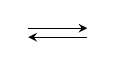
\begin{tikzpicture}[baseline] \draw[>=stealth,->] (0,1ex) -- (0.75,1ex); \draw[>=stealth,->] (0.75,0.25ex) -- (0,0.25ex); \end{tikzpicture}\ {#3}\colon{#4}}

\renewcommand{\to}{\ \tikz[baseline]\draw[>=stealth,->](0,0.5ex)--(0.5,0.5ex);\ }
\newcommand{\ot}{\ \tikz[baseline]\draw[>=stealth,<-](0,0.5ex)--(0.5,0.5ex);\ }

%----------------------------------------------------------------------%

%\hyphenation{Mack-ey mon-oid-al Wald-hau-sen}

%----------------------------------------------------------------------% 




%\usepackage{hyperref}
%\usepackage{color}


%----------------------------------------------------------------------%
\begin{document}
\title{Structured Splittings of $\Omega SU(n)$ and Snaith's Construction of Periodic Complex Bordism}

\author{Jeremy Hahn and Allen Yuan}

%----------------------------------------------------------------------%
%----------------------------------------------------------------------%


\maketitle
\tableofcontents


%----------------------------------------------------------------------%

\section{Introduction}

Write this last after we have filled in all the theorems with complete proofs.

%Notations
%Sp for spectra, S for spaces?
%Disclaimer: Using \infty cats everywhere
\section{Filtered and Graded Ring Spectra}

%Cite Rotation Invariance \cite{LurieRot} and lay out the basic theory.  Explain why an $\mathbb{E}_n$ filtered spectrum with $\mathbb{E}_n$-backwards maps must be split.
%I'd be happy to do this.  It's in progress below, but I'm not great with texing and notation so please give me suggestions.
%should probably write this for a general stable \infty category C
Here we review a framework from \cite{LurieRot} for studying graded and filtered objects.  The reader is referred to \cite{LurieRot} for a more thorough treatment and all proofs.  

Let $\C$ be a stable $\infty$-category.  Denote by $\Z_{\geq 0}$ the poset of non-negative integers, and by $\Z_{\geq 0}^{ds}$ the corresponding discrete category.  The reader is warned that our numbering conventions are opposite the ones in \cite{LurieRot}.  
\begin{dfn} 
Let $\Gr(\C)$ denote the functor category $\Fun(\Z_{\geq 0}^{ds}, \C).$  We shall refer to $\Gr(\C)$ as the category of graded objects in $\C$.  Its objects can be thought of as sequences $X_0, X_1,X_2,\cdots \in \C$.  
\end{dfn}
\begin{dfn} 
Let $\Fil(\C)$ denote the functor category $\Fun(\Z_{\geq 0}, \C).$  We shall refer to $\Fil$ as the category of filtered spectra.  Its objects can be thought of as sequences $Y_0\to Y_1\to Y_2 \to \cdots$ of spectra filtering $\colim_i Y_i$.  
\end{dfn}

%paragraph describes the functors
The obvious map $\Z_{\geq 0}^{ds} \to \Z_{\geq 0}$ induces a restriction functor $\text{res}: \Fil \to \Gr.$  The restriction is right adjoint to a functor $I: \Gr \to \Fil$ given by left Kan extension.  The functor $I$ can be thought of as taking a graded spectrum $X_0,X_1,X_2,\cdots$ to the filtered spectrum $X_0\to X_0\oplus X_1\to X_0\oplus X_1\oplus X_2\to \cdots.$    There is also an associated graded functor $\text{gr }: \Fil \to \Gr$ such that the composite $\text{gr }\circ I : \Gr \to \Gr$ is an equivalence.   

%paragraph describes the monoidal structures
The categories $\Gr$ and $\Fil$ are given symmetric monoidal structures via the Day convolution; we denote the operation in both cases by $\otimes$.  The unit $\S0^{gr}$ of $\otimes$ in graded spectra is $S^0$ in degree 0 and $*$ otherwise; the unit $\S0^{fil}$ in filtered spectra is $I\S0^{gr}.$  

The functors $I$ and $\text{gr}$ can be given symmetric monoidal structures such that the composite $\text{gr }\circ I : \Gr \to \Gr$ is a symmetric monoidal equivalence.  It follows in particular that they extend to functors on between the categories of $\E_n$ algebras in $\Gr$ and $\Fil$.  Thus, given an $\E_n$ algebra $Y$ in filtered spectra, we obtain a canonical $\E_n$ structure on its associated graded $\text{gr}(Y).$  Conversely, given $X\in \Alg_{\E_n}(\Fil)$


%, and thus induces a functor $I:\Alg_{\E_n}(\Gr)\to \Alg_{\E_n}(\Fil).$   Similarly, the functor $\text{gr}$ can be given a symmetric monoidal structure such that the 
%As such, it makes sense to talk about $\mathbb{E}_n$ algebras in $\Fil$ and $\Gr$.  In fact, 

%maybe we should set apart the definitions that jacob did not already make?
\begin{dfn}
An object $X\in \Alg_{\E_n}(\Fil)$ is called \emph{$\E_n$-split} if it is in the essential image of $I$.  
\end{dfn}

Given an $\E_n$-split filtered spectrum $X$, we can recover the underlying graded spectrum by taking the associated graded. 


\section{The (Segal-Mitchell-Richter?) Filtration on $\Omega SU(n)$}

I believe Mitchell shows in \cite{MitchellSU(n)} that the filtration is filtered $\mathbb{A}_\infty$.  We need to check this.

\begin{cnj} The filtration is $\mathbb{E}_2$.
\end{cnj}
I guess now we know this is just true.  We should probably thank Jacob for bringing to our attention that this conjecture of Mahowald is actually well-known by geometric representation theorists.  
%We can leave this as a conjecture if we don't make easy progress on it.  Seems potentially hard.  We should cite Rotation Invariance for the $n \rightarrow \infty$ case and explain that our conjecture would be a refinement of the one in \cite{MahowaldRichter}.  It might also be worth briefly digging into \cite{MitchellLoopGroup} to see if our arguments generalize to broader loop group contexts.  We could also see if the splitting of all loops of Steifel manifolds is $\mathbb{A}_\infty$-structure, and not just $\Omega SU(n)$.  We can always write a sequel to this preprint if we feel like it.

\section{An $\mathbb{A}_\infty$-splitting by Weiss Calculus}


In this section, we extend the methods of \cite{Arone} to produce $\mathbb{A}_\infty$ stable splittings of Stiefel manifolds.  
%some sort of outline
%Review of weiss calculus
%monoidalness of Weiss Calculus
%general splitting machinery
\subsection{Weiss Calculus}
%cite Weiss
Let $\J$ be the $\infty$-category which is the nerve of the topological category whose objects are finite dimensional complex vector spaces equipped with a Hermitian inner product and whose morphisms are spaces of linear isometries.  


\subsection{General splitting machinery}


Let $[n]$ denote the linearly ordered set of integers $0\leq i\leq n$.  Define $\Fil_n = \text{Fun}([n], \Sp^{\J})$ and $\Cofil_n = \text{Fun}([n]^{\text{op}},\Sp^{\J})$.  These categories admit functors to $\Sp^{\J}$ by taking colimit and limit, respectively.  Let $\C_n = \Fil_n \times_{\Sp^{\J}} \Cofil_n.$  Finally, let $\Gr_n = \text{Fun}([n]^{\text{ds}}, \Sp^{\J})$ where $[n]^{\text{ds}}$ denotes the underlying discrete category.  We have the following lemma:

\begin{lem}
For all integers $n>0$, there is a fully faithful functor $i_n:\Gr_{n+1} \to \C_n.$  
\end{lem}
\begin{proof}
An element of $\C_n$ is given by a sequence of maps 

The proof is by induction.  
\end{proof}

We may then take inverse limits to get a category $\C_\infty = \Fil(\Sp^{\J}) \times_{\Sp^{\J}} \Cofil(\Sp^{\J})$ and a functor $i: \Gr \to \C_\infty$. 

\begin{cor}
The functor $i$ is fully faithful.
\end{cor}
\begin{proof}
%This amounts to checking that taking inverse limits retains fully faithfulness.  I think this is totally obvious if you were taking an inverse limit of simplicial sets, but maybe we need to be a little careful since we want a homotopy limit?
\end{proof}


at the end, restrict connectivity so that it's monoidal








\section{An $\mathbb{E}_2$-splitting in Complex Cobordism}

Let $R$ denote any $\mathbb{E}_2$-ring spectrum with even-concentrated homotopy groups.  I claim that any $\mathbb{A}_\infty$-morphism $\Omega SU(n) \rightarrow R$ lifts to an $\mathbb{E}_2$-morphism.

The argument is inspired by \cite{ChadwickMandell}
\begin{proof}
The obstructions live in $H_*(\Omega SU(n);\pi_{*+1}(R))$, and no matter the value of $\pi_{*+1}(R)$ this is $0$.
\end{proof}

\begin{cor}
If $R$ is the relevant split $MU$-$\mathbb{E}_2$-algebra, this yields an $MU$-$\mathbb{E}_2$-algebra equivalence $\Omega SU(n) \smsh MU \rightarrow R$ by adjunction from the $\mathbb{E}_2$-map $\Omega SU(n) \rightarrow R$.
\end{cor}

\section{Obstructions to a general $\mathbb{E}_2$-splitting}

Suppose there is a map $\Sigma^{\infty}_+ \Omega SU(n) \rightarrow \Sigma^{\infty}_+ \mathbb{CP}^{n-1}$.  This is adjoint to a double loop map $\Omega SU(n) \rightarrow GL_1(\Sigma^{\infty}_+\mathbb{CP}^{n-1})$ which lands in the component $SL_1(\Sigma^{\infty}_+ \mathbb{CP}^{n-1}) \simeq \Omega^2 \Sigma^2 \mathbb{CP}^{n-1}$.  BLAH BLAH
%maybe remark that BU -> QCP^\infty not being E_2 is still true after taking \Sigma^\infty_+, and remark that this is like a version of the splitting principle.

\section{Snaith's Construction of Periodic Complex Bordism}

A classical theorem of Snaith \cite{SnaithOriginal} gives an equivalence of homotopy commutative ring spectra $$\Sigma^{\infty}_+ BU [\beta^{-1}] \simeq MUP.$$  The equivalence arises from considering the total $MU$-Chern class map $BU \to GL_1(MUP).$  It is known from \cite{SnaithNotMultiplicative} that the total Chern class in integral homology is not an infinite loop map.  It follows from the existence of an $\E_\infty$ map $MUP \to H\Z P$ from periodic complex bordism to periodic integral homology that Snaith's equivalence is not an equivalence of $\E_\infty$ ring spectra.  The following theorem refines this observation:


%should check if the obstruction in SnaithNotMultiplicative is also E_3...I would think it is
%should we also cite the totaro paper that does literally the same thing as SnaithNotMultiplicative?

\begin{thm}
The equivalence $\Sigma^{\infty}_+ BU [\beta^{-1}] \simeq MUP$ is $\mathbb{E}_2$ but not $\mathbb{E}_3$.
\end{thm}

\begin{proof}
Proof goes here
\end{proof}

Comment now about GepnerSnaith.
We should cite at some point here or the introduction all of \cite{SnaithNotMultiplicative},  \cite{GepnerSnaith}, and the Snaith book with the original splitting.

\section{Miscellaneous stuff here}

It would be nice to at some point deal with showing the associated graded $E_2$ structure of BU is the thom spectrum VMU(n).  I've directly pasted in some writing from a previous argument I claimed, but it definitely uses that $\coprod BU(n)$ is an $E_2$ algebra over $\Z _{\geq 0}$ which I never got straight an actual proof of.  

\begin{prop}The associated graded of $\Sigma^{\infty}_+BU$ is $E_2$ equivalent to the Thom spectrum $\bigvee MU(n).$
\end{prop}
\begin{proof}
Let $R = BU$ with its natural filtration, and let $R^{\oplus} = \coprod BU(n)$ with its natural filtration.  Let $M$ be the ($E_\infty$) filtered spectrum which is $MU(n)$ in degree $n$, and all maps are $0$.  In other words, $\bigvee MU(n)$ with its natural filtration is $I(res(M))$.  

We begin with a filtered $E_\infty$ map $z:R^\oplus \to I(res(M))$ coming from the zero section.  Then, $R^\oplus$ comes with the structure of an $E_2$ algebra over $\Z_{\geq 0}^{fil}$.  In fact, $I(res(M))$  has a trivial structure as an $E_\infty$-algebra over $\Z_{\geq 0}^{fil}$ via the augmentation $\Z_{\geq 0}^{fil}\to S^{0,fil} \to I(res(M))$.  We may then tensor $z$ along the augmentation to get a map of $E_2$ filtered spectra $z':R \to I(res(M))$.  

There is a canonical equivalence $I(res(M)) \otimes \mathbb{A} \simeq M$ because $M$ is in the image of $\mathbb{A} \otimes I(-)$ (that is, all the maps in the filtration of $M$ were zero).  As such, $M$ acquires a canonical structure as an $\mathbb{A}$ algebra such that the map $M \otimes \mathbb{A} \to M$ is a map of $E_2$ rings (in fact I think it's $E_\infty$?).  

Finally, we observe that we may tensor $z'$ with $\mathbb{A}$ and compose with the multiplication map to get an $E_2$ map $R\otimes A \to M \otimes A \to M$ which is the right thing up to homotopy, so it's an equivalence.  
\end{proof}

******  

What is $\Sigma^{\infty}_+ \Omega SU(n)[\beta^{-1}]$, by the way?  Is it related to a periodic version of the $X(n)$-filtration of $MU$??
\bibliographystyle{amsalpha}
\bibliography{Bibliography}

\end{document}